\begin{figure}[H]
    \centering
    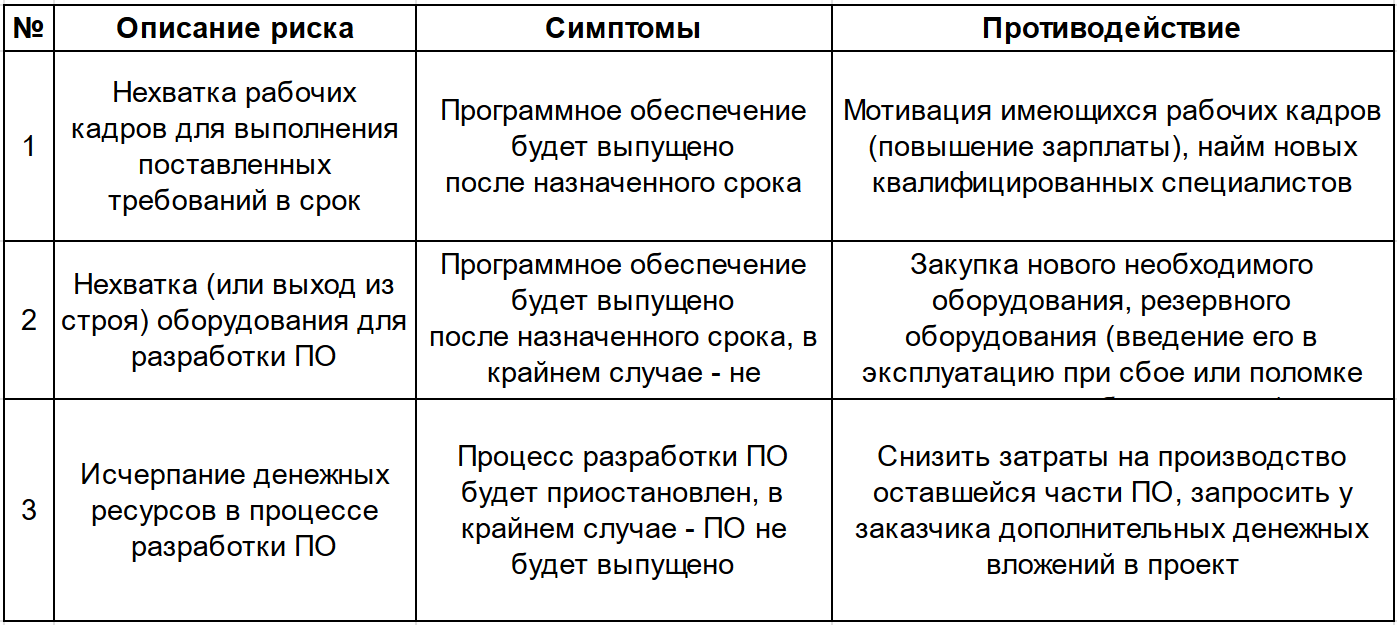
\includegraphics[width=\textwidth]{res/danger-res.png}
    % \caption{Оценка ресурсных рисков рисков.}
    \label{fig:danger-res}
\end{figure}


% \begin{tabular}{|c|c|c|c|}
% №	&	Описание риска	&	Симптомы	&	Противодействие	\\	\hline
% 1	&	Нехватка рабочих кадров для выполнения поставленных требований в срок	&	"Программное обеспечение будет выпущено 
% после назначенного срока"	&	Мотивация имеющихся рабочих кадров (повышение зарплаты), найм новых квалифицированных специалистов	\\	\hline
% 2	&	Нехватка (или выход из строя) оборудования для разработки ПО	&	"Программное обеспечение будет выпущено 
% после назначенного срока, в крайнем случае - не выпущено"	&	Закупка нового необходимого оборудования, резервного оборудования (введение его в эксплуатацию при сбое или поломке основного оборудования)	\\	\hline
% 3	&	Исчерпание денежных ресурсов в процессе разработки ПО	&	Процесс разработки ПО будет приостановлен, в крайнем случае - ПО не будет выпущено	&	Снизить затраты на производство оставшейся части ПО, запросить у заказчика дополнительных денежных вложений в проект	\\	\hline
% \end{tabular}